\documentclass[11pt,oneside]{article}
\usepackage[T1]{fontenc}
\usepackage[utf8]{inputenc}
%\usepackage[latin1]{inputenc}
\DeclareUnicodeCharacter{00A0}{ }
% \usepackage{lmodern}
%\usepackage[adobe-utopia,uppercase=upright,greeklowercase=upright]{mathdesign}
\usepackage[adobe-utopia]{mathdesign}
%\usepackage{minionpro}
% \usepackage{pifont}
% \usepackage{amssymb}
\usepackage{amsmath}
\usepackage[francais]{babel}
% \usepackage[francais]{varioref}
\usepackage[dvips]{graphicx}
\usepackage{here}
\usepackage{framed}
\usepackage[normalem]{ulem}
\usepackage{fancyhdr}
\usepackage{titlesec}
\usepackage{vmargin}
\usepackage{longtable}

\usepackage{amsmath}

\usepackage{ifthen}
%\usepackage[•]{caption}

%\usepackage{epsfig}
\usepackage{subfig}

\usepackage{multirow}
\usepackage{multicol} % Portions de texte en colonnes
\usepackage{flafter}%floatants après la référence



\usepackage{color}
\usepackage{colortbl}


\definecolor{gris25}{gray}{0.75}
\definecolor{bleu}{RGB}{18,33,98}
\definecolor{bleuf}{RGB}{42,94,171}
\definecolor{bleuc}{RGB}{231,239,247}
\definecolor{rougef}{RGB}{185,18,27}
\definecolor{rougec}{RGB}{255,230,231}
\definecolor{vertf}{RGB}{103,126,82}
\definecolor{vertc}{RGB}{220,255,191}
\definecolor{violetf}{RGB}{112,48,160}
\definecolor{violetc}{RGB}{230,224,236}
\definecolor{jaunec}{RGB}{220,255,191}

\newenvironment{sci}[1][\hsize]%
{%
    \def\FrameCommand%
    {%
%\rotatebox{90}{\textit{\textsf{Scilab}}
\includegraphics[height=.8cm]{png/logo_scilab}} 
\rotatebox{90}{
\includegraphics[height=.6cm]{png/logo_scilab}} 
        {\color{violetf}\vrule width 3pt}%
        \hspace{0pt}%must no space.
        \fboxsep=\FrameSep\colorbox{violetc}%
    }%
    \MakeFramed{\hsize #1 \advance\hsize-\width\FrameRestore}%
}%
{\endMakeFramed}%

\newenvironment{pseudo}[1][\hsize]%
{%
    \def\FrameCommand%
    {%
\rotatebox{90}{\textit{\textsf{Pseudo Code}}} 
        {\color{violetf}\vrule width 3pt}%
        \hspace{0pt}%must no space.
        \fboxsep=\FrameSep\colorbox{violetc}%
    }%
    \MakeFramed{\hsize #1 \advance\hsize-\width\FrameRestore}%
}%
{\endMakeFramed}%

\newenvironment{py}[1][\hsize]%
{%
    \def\FrameCommand%
    {%
%\rotatebox{90}{\textit{\textsf{Python}}} 
\rotatebox{90}{
\includegraphics[height=.6cm]{png/logo_python}} 
        {\color{violetf}\vrule width 3pt}%
        \hspace{0pt}%must no space.
        \fboxsep=\FrameSep\colorbox{violetc}%
    }%
    \MakeFramed{\hsize #1 \advance\hsize-\width\FrameRestore}%
}%
{\endMakeFramed}%


\newenvironment{term}[1][\hsize]%
{%
    \def\FrameCommand%
    {%
\rotatebox{90}{\textit{\textsf{Terminal}}} 
        {\color{violetf}\vrule width 3pt}%
        \hspace{0pt}%must no space.
        \fboxsep=\FrameSep\colorbox{violetc}%
    }%
    \MakeFramed{\hsize #1 \advance\hsize-\width\FrameRestore}%
}%
{\endMakeFramed}%


\newenvironment{rem}[1][\hsize]%
{%
    \def\FrameCommand
    {%
\rotatebox{90}{\textit{\textsf{Remarque}}} 
        {\color{bleuf}\vrule width 3pt}%
        \hspace{0pt}%must no space.
        \fboxsep=\FrameSep\colorbox{bleuc}%
    }%
    \MakeFramed{\hsize#1\advance\hsize-\width\FrameRestore}%
}%
{\endMakeFramed}%


\newenvironment{savoir}[1][\hsize]%
{%
    \def\FrameCommand
    {%
\rotatebox{90}{\textit{\textsf{Savoir}}} 
        {\color{bleuf}\vrule width 3pt}%
        \hspace{0pt}%must no space.
        \fboxsep=\FrameSep\colorbox{bleuc}%
    }%
    \MakeFramed{\hsize#1\advance\hsize-\width\FrameRestore}%
}%
{\endMakeFramed}%

\newenvironment{objectif}[1][\hsize]%
{%
    \def\FrameCommand
    {%
\rotatebox{90}{\textit{\textsf{Objectif}}} 
        {\color{rougef}\vrule width 3pt}%
        \hspace{0pt}%must no space.
        \fboxsep=\FrameSep\colorbox{rougec}%
    }%
    \MakeFramed{\hsize#1\advance\hsize-\width\FrameRestore}%
}%
{\endMakeFramed}%

\newenvironment{prob}[1][\hsize]%
{%
    \def\FrameCommand%
    {%
\rotatebox{90}{\textit{\textsf{ Problématique}}} 
        {\color{rougef}\vrule width 3pt}%
        \hspace{0pt}%must no space.
        \fboxsep=\FrameSep\colorbox{rougec}%
    }%
    \MakeFramed{\hsize#1\advance\hsize-\width\FrameRestore}%
}%
{\endMakeFramed}%

\newenvironment{obj}[1][\hsize]%
{%
    \def\FrameCommand%
    {%
\rotatebox{90}{\textit{\textsf{ $\;$}}} 
        {\color{rougef}\vrule width 3pt}%
        \hspace{0pt}%must no space.
        \fboxsep=\FrameSep\colorbox{rougec}%
    }%
    \MakeFramed{\hsize#1\advance\hsize-\width\FrameRestore}%
}%
{\endMakeFramed}%

\newenvironment{defi}[1][\hsize]%
{%
    \def\FrameCommand%
    {%
\rotatebox{90}{\textit{\textsf{Définition\\}}} 
        {\color{bleuf}\vrule width 3pt}%
        \hspace{0pt}%must no space.
        \fboxsep=\FrameSep\colorbox{bleuc}%
    }%
    \MakeFramed{\hsize#1\advance\hsize-\width\FrameRestore}%
}%
{\endMakeFramed}%


\newenvironment{demo}[1][\hsize]%
{%
    \def\FrameCommand%
    {%
\rotatebox{90}{\textit{\textsf{Démonstration\\}}} 
        {\color{bleuf}\vrule width 3pt}%
        \hspace{0pt}%must no space.
        \fboxsep=\FrameSep\colorbox{bleuc}%
    }%
    \MakeFramed{\hsize#1\advance\hsize-\width\FrameRestore}%
}%
{\endMakeFramed}%


\newenvironment{hypo}[1][\hsize]%
{%
    \def\FrameCommand%
    {%
\rotatebox{90}{\textit{\textsf{Hypothèse\\}}} 
        {\color{bleuf}\vrule width 3pt}%
        \hspace{0pt}%must no space.
        \fboxsep=\FrameSep\colorbox{bleuc}%
    }%
    \MakeFramed{\hsize#1\advance\hsize-\width\FrameRestore}%
}%
{\endMakeFramed}%


\newenvironment{prop}[1][\hsize]%
{%
    \def\FrameCommand%
    {%
\rotatebox{90}{\textit{\textsf{Propriété\\}}} 
        {\color{bleuf}\vrule width 3pt}%
        \hspace{0pt}%must no space.
        \fboxsep=\FrameSep\colorbox{bleuc}%
    }%
    \MakeFramed{\hsize#1\advance\hsize-\width\FrameRestore}%
}%
{\endMakeFramed}%

\newenvironment{props}[1][\hsize]%
{%
    \def\FrameCommand%
    {%
\rotatebox{90}{\textit{\textsf{Propriétés\\}}} 
        {\color{bleuf}\vrule width 3pt}%
        \hspace{0pt}%must no space.
        \fboxsep=\FrameSep\colorbox{bleuc}%
    }%
    \MakeFramed{\hsize#1\advance\hsize-\width\FrameRestore}%
}%
{\endMakeFramed}%

\newenvironment{exemple}[1][\hsize]%
{%
    \def\FrameCommand%
    {%
\rotatebox{90}{\textit{\textsf{Exemple\\}}} 
        {\color{vertf}\vrule width 3pt}%
        \hspace{0pt}%must no space.
        \fboxsep=\FrameSep\colorbox{vertc}%
    }%
    \MakeFramed{\hsize#1\advance\hsize-\width\FrameRestore}%
}%
{\endMakeFramed}%

\newenvironment{exercice}[1][\hsize]%
{%
    \def\FrameCommand%
    {%
\rotatebox{90}{\textit{\textsf{Exercice\\}}} 
        {\color{vertf}\vrule width 3pt}%
        \hspace{0pt}%must no space.
        \fboxsep=\FrameSep\colorbox{vertc}%
    }%
    \MakeFramed{\hsize#1\advance\hsize-\width\FrameRestore}%
}%
{\endMakeFramed}%

\newenvironment{Support}[1][\hsize]%
{%
    \def\FrameCommand%
    {%
\rotatebox{90}{\textit{\textsf{Support de cours\\}}} 
        {\color{vertf}\vrule width 3pt}%
        \hspace{0pt}%must no space.
        \fboxsep=\FrameSep\colorbox{jaunec}%
    }%
    \MakeFramed{\hsize#1\advance\hsize-\width\FrameRestore}%
}%
{\endMakeFramed}%

\newenvironment{resultat}[1][\hsize]%
{%
    \def\FrameCommand%
    {%
\rotatebox{90}{\textit{\textsf{Résultat\\}}} 
        {\color{rougef}\vrule width 3pt}%
        \hspace{0pt}%must no space.
        \fboxsep=\FrameSep\colorbox{rougec}%
    }%
    \MakeFramed{\hsize#1\advance\hsize-\width\FrameRestore}%
}%
{\endMakeFramed}%

\newenvironment{methode}[1][\hsize]%
{%
    \def\FrameCommand%
    {%
\rotatebox{90}{\textit{\textsf{Méthode\\}}} 
        {\color{rougef}\vrule width 3pt}%
        \hspace{0pt}%must no space.
        \fboxsep=\FrameSep\colorbox{rougec}%
    }%
    \MakeFramed{\hsize#1\advance\hsize-\width\FrameRestore}%
}%
{\endMakeFramed}%

\newenvironment{theo}[1][\hsize]%
{%
    \def\FrameCommand%
    {%
\rotatebox{90}{\textit{\textsf{Théorème\\}}} 
        {\color{rougef}\vrule width 3pt}%
        \hspace{0pt}%must no space.
        \fboxsep=\FrameSep\colorbox{rougec}%
    }%
    \MakeFramed{\hsize#1\advance\hsize-\width\FrameRestore}%
}%
{\endMakeFramed}%

\newenvironment{warn}[1][\hsize]%
{%
    \def\FrameCommand%
    {%
\rotatebox{90}{\textit{\textsf{Attention\\}}} 
        {\color{rougef}\vrule width 3pt}%
        \hspace{0pt}%must no space.
        \fboxsep=\FrameSep\colorbox{rougec}%
    }%
    \MakeFramed{\hsize#1\advance\hsize-\width\FrameRestore}%
}%
{\endMakeFramed}%

% \usepackage{pstricks}
%\usepackage{minitoc}
% \setcounter{minitocdepth}{4}

\setcounter{tocdepth}{2}

% \mtcselectlanguage{french} 

%\usepackage{draftcopy}% "Brouillon"
% \usepackage{floatflt}
\usepackage{psfrag}
%\usepackage{listings} % Permet d'insérer du code de programmation
\renewcommand{\baselinestretch}{1.2}

% Changer la numérotation des figures :
% ------------------------------------
% \makeatletter
% \renewcommand{\thefigure}{\ifnum \c@section>\z@ \thesection.\fi
%  \@arabic\c@figure}
% \@addtoreset{figure}{section}
% \makeatother
 


%%%%%%%%%%%%
% Définition des vecteurs %
%%%%%%%%%%%%
 \newcommand{\vect}[1]{\overrightarrow{#1}}

%%%%%%%%%%%%
% Définition des torseusr %
%%%%%%%%%%%%

 \newcommand{\torseur}[1]{%
\left\{{#1}\right\}
}

\newcommand{\torseurcin}[3]{%
\left\{\mathcal{#1} \left(#2/#3 \right) \right\}
}

\newcommand{\torseurstat}[3]{%
\left\{\mathcal{#1} \left(#2\rightarrow #3 \right) \right\}
}

 \newcommand{\torseurc}[8]{%
%\left\{#1 \right\}=
\left\{
{#1}
\right\}
 = 
\left\{%
\begin{array}{cc}%
{#2} & {#5}\\%
{#3} & {#6}\\%
{#4} & {#7}\\%
\end{array}%
\right\}_{#8}%
}

 \newcommand{\torseurcol}[7]{
\left\{%
\begin{array}{cc}%
{#1} & {#4}\\%
{#2} & {#5}\\%
{#3} & {#6}\\%
\end{array}%
\right\}_{#7}%
}

 \newcommand{\torseurl}[3]{%
%\left\{\mathcal{#1}\right\}_{#2}=%
\left\{%
\begin{array}{l}%
{#1} \\%
{#2} %
\end{array}%
\right\}_{#3}%
}

 \newcommand{\vectv}[3]{%
\vect{V\left( {#1} \in {#2}/{#3}\right)}
}


\newcommand{\vectf}[2]{%
\vect{R\left( {#1} \rightarrow {#2}\right)}
}

\newcommand{\vectm}[3]{%
\vect{\mathcal{M}\left( {#1}, {#2} \rightarrow {#3}\right)}
}


 \newcommand{\vectg}[3]{%
\vect{\Gamma \left( {#1} \in {#2}/{#3}\right)}
}

 \newcommand{\vecto}[2]{%
\vect{\Omega\left( {#1}/{#2}\right)}
}
% }$$\left\{\mathcal{#1} \right\}_{#2} =%
% \left\{%
% \begin{array}{c}%
%  #3 \\%
%  #4 %
% \end{array}%
% \right\}_{#5}}

%  ------------------------------------------
% | Modification du formatage des sections : | 
%  ------------------------------------------

% Grands titres :
% ---------------

\newcommand{\titre}[1]{%
\begin{center}
      \bigskip
      \rule{\textwidth}{1pt}
      \par\vspace{0.1cm}
      
      \textbf{\large #1}
      \par\rule{\textwidth}{1pt}
    \end{center}
    \bigskip
  }

% Supprime le numéro du chapitre dans la numérotation des sections:
% -----------------------------------------------------------------
\makeatletter
\renewcommand{\thesection}{\@arabic\c@section}
\makeatother


% \titleformat{\chapter}[display]
% {\normalfont\Large\filcenter}
% {}
% {1pc}
% {\titlerule[1pt]
%   \vspace{1pc}%
%   \Huge}[\vspace{1ex}%
% \titlerule]


%%%% Chapitres Comme PY Pechard %%%%%%%%%
% numéro du chapitre
\DeclareFixedFont{\chapnumfont}{OT1}{phv}{b}{n}{80pt}
% pour le mot « Chapitre »
\DeclareFixedFont{\chapchapfont}{OT1}{phv}{m}{it}{40pt}
% pour le titre
\DeclareFixedFont{\chaptitfont}{T1}{phv}{b}{n}{25pt}

\definecolor{gris}{gray}{0.75}
\titleformat{\chapter}[display]%
	{\sffamily}%
	{\filleft\chapchapfont\color{gris}\chaptertitlename\
	\\
	\vspace{12pt}
	\chapnumfont\thechapter}%
	{16pt}%
	{\filleft\chaptitfont}%
	[\vspace{6pt}\titlerule\titlerule\titlerule]

%%%%  Fin Chapitres Comme PY Pechard %%%%%%%%%


% Section, subsection, subsubsection sans serifs :
% % ----------------------------------------------

% \makeatletter
% \renewcommand{\section}{\@startsection{section}{0}{0mm}%
% {\baselineskip}{.3\baselineskip}%
% {\normalfont\sffamily\Large\textbf}}%
% \makeatother

\makeatletter
\renewcommand{\@seccntformat}[1]{{\textcolor{bleu}{\csname
the#1\endcsname}\hspace{0.5em}}}
\makeatother

\makeatletter
\renewcommand{\section}{\@startsection{section}{1}{\z@}%
                       {-4ex \@plus -1ex \@minus -.4ex}%
                       {1ex \@plus.2ex }%
                       {\normalfont\Large\sffamily\bfseries}}%
\makeatother
 
\makeatletter
\renewcommand{\subsection}{\@startsection {subsection}{2}{\z@}
                          {-3ex \@plus -0.1ex \@minus -.4ex}%
                          {0.5ex \@plus.2ex }%
                          {\normalfont\large\sffamily\bfseries}}
\makeatother
 
\makeatletter
\renewcommand{\subsubsection}{\@startsection {subsubsection}{3}{\z@}
                          {-2ex \@plus -0.1ex \@minus -.2ex}%
                          {0.2ex \@plus.2ex }%
                          {\normalfont\large\sffamily\bfseries}}
\makeatother
 
\makeatletter             
\renewcommand{\paragraph}{\@startsection{paragraph}{4}{\z@}%
                                    {-2ex \@plus-.2ex \@minus .2ex}%
                                    {0.1ex}%               
{\normalfont\sffamily\bfseries}}
\makeatother
 
 
\makeatletter             
\renewcommand{\subparagraph}{\@startsection{subparagraph}{5}{\z@}%
                                    {-2ex \@plus-.2ex \@minus .2ex}%
                                    {0ex}%               
{\normalfont\bfseries Question }}
\makeatother
\renewcommand{\thesubparagraph}{\arabic{subparagraph}} 
\makeatletter


\renewcommand{\thesubparagraph}{\arabic{subparagraph}} 

% \makeatletter
% \renewcommand{\subsection}{\@startsection{subsection}{1}{2mm}%
% {\baselineskip}{.3\baselineskip}%
% {\normalfont\sffamily\large\textbf}}%
% \makeatother
% 
% \makeatletter
% \renewcommand{\subsubsection}{\@startsection{subsubsection}{2}{4mm}%
% {\baselineskip}{.15\baselineskip}%
% {\normalfont\sffamily\large\textbf}}%
% \makeatother
% 
% \makeatletter
% \renewcommand{\paragraph}{\@startsection{paragraph}{3}{6mm}%
% {\baselineskip}{.15\baselineskip}%
% {\normalfont\sffamily\large\textbf}}%
% \makeatother
 
\setcounter{secnumdepth}{5}


%  --------
% | Marges |
%  --------


% \setmarginsrb{2.5cm}{1.5cm}{2.5cm}{2cm}{1cm}{1cm}{1cm}{1cm}
\setmarginsrb{1.5cm}{1cm}{1cm}{1.5cm}{1cm}{1cm}{1cm}{1cm}

% Changer les marges localement :
% -----------------------------
\newenvironment{changemargin}[2]{\begin{list}{}{%
\setlength{\topsep}{0pt}%
\setlength{\leftmargin}{0pt}%
\setlength{\rightmargin}{0pt}%
\setlength{\listparindent}{\parindent}%
\setlength{\itemindent}{\parindent}%
\setlength{\parsep}{0pt plus 1pt}%
\addtolength{\leftmargin}{#1}%
\addtolength{\rightmargin}{#2}%
}\item }{\end{list}}



\usepackage{pst-solides3d}
\usepackage{titletoc}
\titlecontents{chapter}[+3pc]
  {\addvspace{10pt}\sffamily\bfseries}
{\contentslabel[{\pscirclebox[fillstyle=solid,fillcolor=gray!25,
linecolor=gray!25,framesep=4pt]{\textcolor{white}{\thecontentslabel}}}]{2.5pc}}
  {}
  {\dotfill \normalfont\thecontentspage\ }

\titlecontents{section}[3pc]
  {\addvspace{2pt}\sffamily}
  {\contentslabel[\thecontentslabel]{1.8pc}}
  {}
  {\dotfill \normalfont\thecontentspage\ }

\titlecontents{subsection}[5pc]
  {\addvspace{2pt}\sffamily}
  {\contentslabel[\thecontentslabel]{1.8pc}}
  {}
  {\dotfill \normalfont\thecontentspage\ }

\titlecontents{subsubsection}[8pc]
  {\addvspace{2pt}\sffamily}
  {\contentslabel[\thecontentslabel]{3pc}}
  {}
  {\dotfill \normalfont\thecontentspage\ }
%{\;\titlerule\;\normalfont\thecontentspage\ }

\titlecontents{paragraph}[9pc]
  {\addvspace{2pt}\sffamily}
  {\contentslabel[\thecontentslabel]{3.5pc}}
  {}
  {\dotfill \normalfont\thecontentspage\ }

%pour avoir l indentation dans minipage
\newdimen\oldparindent\oldparindent=\parindent

\makeatletter
\def\@iiiminipage#1#2[#3]#4{%
  \noindent
  \leavevmode
  \@pboxswfalse
  \setlength\@tempdima{#4}%
  \def\@mpargs{{#1}{#2}[#3]{#4}}%
  \setbox\@tempboxa\vbox\bgroup
    \color@begingroup
      \hsize\@tempdima
      \textwidth\hsize \columnwidth\hsize
      \@parboxrestore
      \parindent=\oldparindent
      \def\@mpfn{mpfootnote}\def\thempfn{\thempfootnote}\c@mpfootnote\z@
      \let\@footnotetext\@mpfootnotetext
      \let\@listdepth\@mplistdepth \@mplistdepth\z@
      \@minipagerestore
      \@setminipage}
\makeatother

%\usepackage{algorithm}
%\usepackage{algorithmic}
\usepackage[french]{algorithm2e}

\SetKwBlock{Fonction}{Début Fonction}{Fin Fonction}
\SetKwComment{Comment}{start}{end}
\SetKwFor{While}{Tant que}{Faire}{Fin tant que}
\SetKwIF{If}{ElseIf}{Else}{Si}{Alors}{Sinon si}{Sinon}{Fin si}
% Python sources

\usepackage{listings}
\lstloadlanguages{R}   % pour regler les pb d accent utf8 dans les codes
\lstset{language=R} % pour regler les pb d accent utf8 dans les codes

\usepackage{textcomp}
\usepackage{setspace}
%\usepackage{palatino}

%\usepackage{color}
\definecolor{Bleu}{rgb}{0.1,0.1,1.0}
\definecolor{Noir}{rgb}{0,0,0}
\definecolor{Grau}{rgb}{0.5,0.5,0.5}
\definecolor{DunkelGrau}{rgb}{0.15,0.15,0.15}
\definecolor{Hellbraun}{rgb}{0.5,0.25,0.0}
\definecolor{Magenta}{rgb}{1.0,0.0,1.0}
\definecolor{Gris}{gray}{0.5}
\definecolor{Vert}{rgb}{0,0.5,0}
\definecolor{SourceHintergrund}{rgb}{1,1.0,0.95}


%
\renewcommand{\lstlistlistingname}{Listings}
\renewcommand{\lstlistingname}{Listing}

\lstnewenvironment{python}[1][]{
\lstset{
numbers=left,
%escapeinside={\%*}{*)},
%inputencoding=utf8,   % pour regler les pb d accent utf8 dans les codes
%extendedchars=true,   % pour regler les pb d accent utf8 dans les codes
language=python,
basicstyle=\sffamily\footnotesize, 	
stringstyle=\color{red}, 
showstringspaces=false, 
alsoletter={1234567890},
otherkeywords={\ , \}, \{},
keywordstyle=\color{blue},
emph={access,and,break,class,continue,def,del,elif ,else,
except,exec,finally,for,from,global,if,import,in,i s,
lambda,not,or,pass,print,raise,return,try,while},
emphstyle=\color{black}\bfseries,
emph={[2]True, False, None, self},
emphstyle=[2]\color{green},
emph={[3]from, import, as},
emphstyle=[3]\color{blue},
upquote=true,
columns=flexible, % pour empecher d'avoir un espacement mono
morecomment=[s]{"""}{"""},
commentstyle=\color{Hellbraun}\slshape, 
%emph={[4]1, 2, 3, 4, 5, 6, 7, 8, 9, 0},
emphstyle=[4]\color{blue},
literate=*{:}{{\textcolor{blue}:}}{1}
{=}{{\textcolor{blue}=}}{1}
{-}{{\textcolor{blue}-}}{1}
{+}{{\textcolor{blue}+}}{1}
{*}{{\textcolor{blue}*}}{1}
{!}{{\textcolor{blue}!}}{1}
{(}{{\textcolor{blue}(}}{1}
{)}{{\textcolor{blue})}}{1}
{[}{{\textcolor{blue}[}}{1}
{]}{{\textcolor{blue}]}}{1}
{<}{{\textcolor{blue}<}}{1}
{>}{{\textcolor{blue}>}}{1}
{COMPLETER}{{\textcolor{red}COMPLETER}}{1},
literate=%
            {é}{{\'{e}}}1
            {è}{{\`{e}}}1
            {ê}{{\^{e}}}1
            {ë}{{\¨{e}}}1
            {û}{{\^{u}}}1
            {ù}{{\`{u}}}1
            {â}{{\^{a}}}1
            {à}{{\`{a}}}1
            {î}{{\^{i}}}1
            {ç}{{\c{c}}}1
            {Ç}{{\c{C}}}1
            {É}{{\'{E}}}1
            {Ê}{{\^{E}}}1
            {À}{{\`{A}}}1
            {Â}{{\^{A}}}1
            {Î}{{\^{I}}}1, % pour regler les pb d accent utf8 dans les codes
%framexleftmargin=1mm, framextopmargin=1mm, frame=shadowbox, rulesepcolor=\color{blue},#1
%backgroundcolor=\color{SourceHintergrund}, 
%framexleftmargin=1mm, framexrightmargin=1mm, framextopmargin=1mm, frame=single, framerule=1pt, rulecolor=\color{black},#1
}}{}



\lstnewenvironment{python2}[1][]{
\lstset{
%escapeinside={\%*}{*)},
%inputencoding=utf8,   % pour regler les pb d accent utf8 dans les codes
%extendedchars=true,   % pour regler les pb d accent utf8 dans les codes
language=python,
basicstyle=\sffamily\footnotesize, 	
stringstyle=\color{red}, 
showstringspaces=false, 
alsoletter={1234567890},
otherkeywords={\ , \}, \{},
keywordstyle=\color{blue},
emph={access,and,break,class,continue,def,del,elif ,else,
except,exec,finally,for,from,global,if,import,in,i s,
lambda,not,or,pass,print,raise,return,try,while},
emphstyle=\color{black}\bfseries,
emph={[2]True, False, None, self},
emphstyle=[2]\color{green},
emph={[3]from, import, as},
emphstyle=[3]\color{blue},
upquote=true,
columns=flexible, % pour empecher d'avoir un espacement mono
morecomment=[s]{"""}{"""},
commentstyle=\color{Hellbraun}\slshape, 
%emph={[4]1, 2, 3, 4, 5, 6, 7, 8, 9, 0},
emphstyle=[4]\color{blue},
literate=*{:}{{\textcolor{blue}:}}{1}
{=}{{\textcolor{blue}=}}{1}
{-}{{\textcolor{blue}-}}{1}
{+}{{\textcolor{blue}+}}{1}
{*}{{\textcolor{blue}*}}{1}
{!}{{\textcolor{blue}!}}{1}
{(}{{\textcolor{blue}(}}{1}
{)}{{\textcolor{blue})}}{1}
{[}{{\textcolor{blue}[}}{1}
{]}{{\textcolor{blue}]}}{1}
{<}{{\textcolor{blue}<}}{1}
{>}{{\textcolor{blue}>}}{1}
{COMPLETER}{{\textcolor{red}COMPLETER}}{1},
literate=%
            {é}{{\'{e}}}1
            {è}{{\`{e}}}1
            {ê}{{\^{e}}}1
            {ë}{{\¨{e}}}1
            {û}{{\^{u}}}1
            {ù}{{\`{u}}}1
            {â}{{\^{a}}}1
            {à}{{\`{a}}}1
            {î}{{\^{i}}}1
            {ç}{{\c{c}}}1
            {Ç}{{\c{C}}}1
            {É}{{\'{E}}}1
            {Ê}{{\^{E}}}1
            {À}{{\`{A}}}1
            {Â}{{\^{A}}}1
            {Î}{{\^{I}}}1, % pour regler les pb d accent utf8 dans les codes
%framexleftmargin=1mm, framextopmargin=1mm, frame=shadowbox, rulesepcolor=\color{blue},#1
%backgroundcolor=\color{SourceHintergrund}, 
%framexleftmargin=1mm, framexrightmargin=1mm, framextopmargin=1mm, frame=single, framerule=1pt, rulecolor=\color{black},#1
}}{}

\lstnewenvironment{scilab}[1][]{
\lstset{
language=scilab,
basicstyle=\sffamily\footnotesize, 	
stringstyle=\color{red}, 
showstringspaces=false, 
alsoletter={1234567890},
otherkeywords={\ , \}, \{},
keywordstyle=\color{blue},
emph={access,and,break,class,continue,def,del,elif ,else,
except,exec,finally,for,from,global,if,import,in,i s,
lambda,not,or,pass,print,raise,return,try,while,Debut},
emphstyle=\color{black}\bfseries,
emph={[2]True, False, None, self},
emphstyle=[2]\color{green},
emph={[3]from, import, as},
emphstyle=[3]\color{blue},
upquote=true,
columns=flexible, % pour empecher d'avoir un espacement mono
morecomment=[s]{"""}{"""},
commentstyle=\color{Hellbraun}\slshape, 
%emph={[4]1, 2, 3, 4, 5, 6, 7, 8, 9, 0},
emphstyle=[4]\color{blue},
literate=*{:}{{\textcolor{blue}:}}{1}
{=}{{\textcolor{blue}=}}{1}
{-}{{\textcolor{blue}-}}{1}
{+}{{\textcolor{blue}+}}{1}
{*}{{\textcolor{blue}*}}{1}
{!}{{\textcolor{blue}!}}{1}
{(}{{\textcolor{blue}(}}{1}
{)}{{\textcolor{blue})}}{1}
{[}{{\textcolor{blue}[}}{1}
{]}{{\textcolor{blue}]}}{1}
{<}{{\textcolor{blue}<}}{1}
{>}{{\textcolor{blue}>}}{1},
%framexleftmargin=1mm, framextopmargin=1mm, frame=shadowbox, rulesepcolor=\color{blue},#1
%backgroundcolor=\color{SourceHintergrund}, 
%framexleftmargin=1mm, framexrightmargin=1mm, framextopmargin=1mm, frame=single, framerule=1pt, rulecolor=\color{black},#1
}}{}


\lstdefinestyle{stylepython}{%
escapeinside={\%*}{*)},
inputencoding=utf8,   % pour regler les pb d accent utf8 dans les codes
extendedchars=true,   % pour regler les pb d accent utf8 dans les codes
language=python,
basicstyle=\sffamily\footnotesize, 	
stringstyle=\color{red}, 
showstringspaces=false, 
alsoletter={1234567890},
otherkeywords={\ , \}, \{},
keywordstyle=\color{blue},
emph={access,and,break,class,continue,def,del,elif ,else,
except,exec,finally,for,from,global,if,import,in,i s,
lambda,not,or,pass,print,raise,return,try,while},
emphstyle=\color{black}\bfseries,
emph={[2]True, False, None, self},
emphstyle=[2]\color{green},
emph={[3]from, import, as},
emphstyle=[3]\color{blue},
upquote=true,
columns=flexible, % pour empecher d'avoir un espacement mono
morecomment=[s]{"""}{"""},
commentstyle=\color{Hellbraun}\slshape, 
%emph={[4]1, 2, 3, 4, 5, 6, 7, 8, 9, 0},
emphstyle=[4]\color{blue},
literate=*{:}{{\textcolor{blue}:}}{1}
{=}{{\textcolor{blue}=}}{1}
{-}{{\textcolor{blue}-}}{1}
{+}{{\textcolor{blue}+}}{1}
{*}{{\textcolor{blue}*}}{1}
{!}{{\textcolor{blue}!}}{1}
{(}{{\textcolor{blue}(}}{1}
{)}{{\textcolor{blue})}}{1}
{[}{{\textcolor{blue}[}}{1}
{]}{{\textcolor{blue}]}}{1}
{<}{{\textcolor{blue}<}}{1}
{>}{{\textcolor{blue}>}}{1}
{COMPLETER}{{\textcolor{red}COMPLETER}}{1},
literate=%
            {é}{{\'{e}}}1
            {è}{{\`{e}}}1
            {ê}{{\^{e}}}1
            {ë}{{\¨{e}}}1
            {û}{{\^{u}}}1
            {ù}{{\`{u}}}1
            {â}{{\^{a}}}1
            {à}{{\`{a}}}1
            {î}{{\^{i}}}1
            {ç}{{\c{c}}}1
            {Ç}{{\c{C}}}1
            {É}{{\'{E}}}1
            {Ê}{{\^{E}}}1
            {À}{{\`{A}}}1
            {Â}{{\^{A}}}1
            {Î}{{\^{I}}}1,
%numbers=left,                    % where to put the line-numbers; possible values are (none, left, right)
%numbersep=5pt,                   % how far the line-numbers are from the code
%numberstyle=\tiny\color{mygray}, % the style that is used for the line-numbers
}

%
%\renewcommand{\algorithmicrequire} {\textbf{\textsc{Entrées:}}}
%\renewcommand{\algorithmicensure}  {\textbf{\textsc{Sorties:}}}
%\renewcommand{\algorithmicwhile}   {\textbf{tantque}}
%\renewcommand{\algorithmicdo}      {\textbf{faire}}
%\renewcommand{\algorithmicendwhile}{\textbf{fin tantque}}
%\renewcommand{\algorithmicend}     {\textbf{fin}}
%\renewcommand{\algorithmicif}      {\textbf{si}}
%\renewcommand{\algorithmicendif}   {\textbf{finsi}}
%\renewcommand{\algorithmicelse}    {\textbf{sinon}}
%\renewcommand{\algorithmicthen}    {\textbf{alors}}
%\renewcommand{\algorithmicfor}     {\textbf{pour}}
%\renewcommand{\algorithmicforall}  {\textbf{pour tout}}
%\renewcommand{\algorithmicdo}      {\textbf{faire}}
%\renewcommand{\algorithmicendfor}  {\textbf{fin pour}}
%\renewcommand{\algorithmicloop}    {\textbf{boucler}}
%\renewcommand{\algorithmicendloop} {\textbf{fin boucle}}
%\renewcommand{\algorithmicrepeat}  {\textbf{répéter}}
%\renewcommand{\algorithmicuntil}   {\textbf{jusqu'à}}

\lstnewenvironment{termi}[1][]{
\lstset{
language=scilab,
basicstyle=\sffamily\footnotesize, 	
stringstyle=\color{red}, 
showstringspaces=false, 
alsoletter={1234567890},
otherkeywords={\ , \}, \{},
keywordstyle=\color{blue},
emph={access,and,break,class,continue,def,del,elif ,else,
except,exec,finally,for,from,global,if,import,in,i s,
lambda,not,or,pass,print,raise,return,try,while,Debut},
emphstyle=\color{black}\bfseries,
emph={[2]True, False, None, self},
emphstyle=[2]\color{green},
emph={[3]from, import, as},
emphstyle=[3]\color{blue},
upquote=true,
columns=flexible, % pour empecher d'avoir un espacement mono
morecomment=[s]{"""}{"""},
commentstyle=\color{Hellbraun}\slshape, 
%emph={[4]1, 2, 3, 4, 5, 6, 7, 8, 9, 0},
emphstyle=[4]\color{blue},
literate=*{:}{{\textcolor{blue}:}}{1}
{=}{{\textcolor{blue}=}}{1}
{-}{{\textcolor{blue}-}}{1}
{+}{{\textcolor{blue}+}}{1}
{*}{{\textcolor{blue}*}}{1}
{!}{{\textcolor{blue}!}}{1}
{(}{{\textcolor{blue}(}}{1}
{)}{{\textcolor{blue})}}{1}
{[}{{\textcolor{blue}[}}{1}
{]}{{\textcolor{blue}]}}{1}
{<}{{\textcolor{blue}<}}{1}
{>}{{\textcolor{blue}>}}{1},
%framexleftmargin=1mm, framextopmargin=1mm, frame=shadowbox, rulesepcolor=\color{blue},#1
%backgroundcolor=\color{SourceHintergrund}, 
%framexleftmargin=1mm, framexrightmargin=1mm, framextopmargin=1mm, frame=single, framerule=1pt, rulecolor=\color{black},#1
}}{}


%
%\renewcommand{\algorithmicrequire} {\textbf{\textsc{Entrées:}}}
%\renewcommand{\algorithmicensure}  {\textbf{\textsc{Sorties:}}}
%\renewcommand{\algorithmicwhile}   {\textbf{tantque}}
%\renewcommand{\algorithmicdo}      {\textbf{faire}}
%\renewcommand{\algorithmicendwhile}{\textbf{fin tantque}}
%\renewcommand{\algorithmicend}     {\textbf{fin}}
%\renewcommand{\algorithmicif}      {\textbf{si}}
%\renewcommand{\algorithmicendif}   {\textbf{finsi}}
%\renewcommand{\algorithmicelse}    {\textbf{sinon}}
%\renewcommand{\algorithmicthen}    {\textbf{alors}}
%\renewcommand{\algorithmicfor}     {\textbf{pour}}
%\renewcommand{\algorithmicforall}  {\textbf{pour tout}}
%\renewcommand{\algorithmicdo}      {\textbf{faire}}
%\renewcommand{\algorithmicendfor}  {\textbf{fin pour}}
%\renewcommand{\algorithmicloop}    {\textbf{boucler}}
%\renewcommand{\algorithmicendloop} {\textbf{fin boucle}}
%\renewcommand{\algorithmicrepeat}  {\textbf{répéter}}
%\renewcommand{\algorithmicuntil}   {\textbf{jusqu'à}}
\newboolean{xp}

\def\xxtitre{\ifthenelse{\boolean{xp}}{
Algorithmique \& Programmation}{
Algorithmique \& Programmation }}

\def\xxsoustitre{\ifthenelse{\boolean{xp}}{
Chapitre 3 -- Algorithmes de tri}{
Chapitre 3 -- Algorithmes de tri}}

\def\xxpied{\ifthenelse{\boolean{xp}}{
Cours -- Algorithmique \& Programmation\\
Chapitre 3 -- Algorithmes de tri}{
\xxtitre}}

\usepackage[%
    pdftitle={Représentation des nombres},
    pdfauthor={Xavier Pessoles},
    colorlinks=true,
    linkcolor=blue,
    citecolor=magenta]{hyperref}

\usepackage{pifont}
%\usepackage{lastpage}

% \makeatletter \let\ps@plain\ps@empty \makeatother
%% DEBUT DU DOCUMENT
%% =================
\sloppy
\hyphenpenalty 10000


\colorlet{shadecolor}{orange!15}

\newtheorem{theorem}{Theorem}


\begin{document}


\newboolean{prof}
\setboolean{prof}{true}
% \makeatletter \let\ps@plain\ps@empty \makeatother
%% DEBUT DU DOCUMENT
%% =================




%------------- En tetes et Pieds de Pages ------------


\pagestyle{fancy}
\ifthenelse{\boolean{xp}}{%
\renewcommand{\headrulewidth}{0pt}}{%
\renewcommand{\headrulewidth}{0.2pt}} %pour mettre le trait en haut
%\renewcommand{\headrulewidth}{0.2pt}

\fancyhead{}
\fancyhead[L]{%
\noindent\begin{minipage}[c]{2.6cm}%

\includegraphics[width=2cm]{png/logo_ptsi.png}%
\end{minipage}}


\fancyhead[C]{\rule{12cm}{.5pt}}



\fancyhead[R]{%
\noindent\begin{minipage}[c]{3cm}
\begin{flushright}
\footnotesize{\textit{\textsf{Informatique}}}%
\end{flushright}
\end{minipage}
}



\fancyhead[C]{\rule{12cm}{.5pt}}

\renewcommand{\footrulewidth}{0.2pt}

\fancyfoot[C]{\footnotesize{\bfseries \thepage}}
\fancyfoot[L]{%
\begin{minipage}[c]{.3\linewidth}
\noindent\footnotesize{{\xxauteur}}
\end{minipage}
\ifthenelse{\boolean{xp}}{}{%
\begin{minipage}[c]{.15\linewidth}

\includegraphics[width=2cm]{png/logoCC.png}
\end{minipage}}
}

\ifthenelse{\boolean{prof}}{%
\fancyfoot[R]{\footnotesize{\xxpied}}}

\begin{center}
 \huge\textsc{\xxtitre}
\end{center}

\begin{center}
 \LARGE\textsc{\xxsoustitre}
\end{center}

\vspace{.5cm}


%---------------------------------------------------------------------------

\begin{Objectif}
 
\begin{itemize}
\item Comprendre et analyser un algorithme de tri
\item Évaluer la complexité d'un algorithme de tri
\item Comparer différents algorithmes de tri
\end{itemize}
\end{Objectif}
 
\setlength{\parskip}{0ex plus 0.2ex minus 0ex}
 \renewcommand{\contentsname}{}
 \renewcommand{\baselinestretch}{1}

\tableofcontents

%\newpage

%---------------------------------------------------------------------------
\section{Complexité d'un algorithme de tri}
%---------------------------------------------------------------------------
\subsection{Définition}
%---------------------------------------------------------------------------
\begin{defi}
\noindent
\underline{Ordre de grandeur} :
Soient $f$ et $g$ deux fonctions positives d’une même variable entière $n$. La fonction $f$ est dite
avoir un ordre de grandeur au plus égal à celui de la fonction $g$ s’il existe un entier
strictement positif $k$ et un entier $N$ tels que, pour tout $n \geq N$, on ait $f(n) \leq k g(n)$. 
On écrira $f = O(g)$. Par exemple, les fonctions $f(n) = 3 n^2 – 5 n + 4$ et
$g(n) = n^2$ ont même ordre de grandeur.\\
\\
\noindent
\underline{Complexité} :
On considère un algorithme $A$. On appelle complexité de $A$ tout ordre de grandeur du
nombre d’opérations élémentaires effectuées pendant le déroulement de l’algorithme. On
exprime ce nombre d’opérations en fonction de paramètres entiers associés aux instances à
traiter ; on pourra par exemple exprimer la complexité d’un tri en fonction du nombre de
données à trier. 
\end{defi}

\noindent
Néanmoins, il se peut qu’avec deux jeux de données différents correspondant
aux mêmes paramètres, le nombre d’opérations effectuées ne soit pas le même. Par exemple,
un algorithme de tri pourra être plus rapide s’il s’agit de trier des données déjà triées que s’il
s’agit de données très désordonnées. On peut alors s’intéresser à :

\begin{itemize}
\item la complexité \textbf{dans le pire des cas} : les paramètres avec lesquels on exprime la
complexité étant fixés, on considère le plus grand nombre d’opérations
élémentaires effectuées sur l’ensemble des instances correspondant à ces
paramètres ; on cherche ainsi un majorant de la complexité qui puisse être atteint
dans certains cas ; c’est ce qu’on fait le plus généralement ;
\item la complexité \textbf{dans le meilleur des cas} : les paramètres avec lesquels on exprime la
complexité étant fixés, on considère le plus petit nombre d’opérations élémentaires
effectuées sur l’ensemble des instances correspondant à ces paramètres ; cette
complexité peut venir compléter la précédente mais ne sera jamais suffisante pour
l’utilisateur ;
\item la complexité \textbf{en moyenne} \textit{(pour information)}: les paramètres avec lesquels on exprime la complexité
étant fixés, il faut alors faire la moyenne des nombres d’opérations élémentaires effectuées, moyenne portant sur tous les jeux de données correspondant à ces paramètres. Ce calcul est généralement difficile et souvent même délicat à
formuler car il faut connaître la probabilité de chacun des jeux de données pour effectuer un calcul pertinent de cette moyenne.
\end{itemize}

%---------------------------------------------------------------------------
\subsection{Illustration}
%---------------------------------------------------------------------------
\noindent
Il existe plusieurs types d'algorithmes de tri que l'on peut classer en comparatifs (ce que l'on verra dans ce cours) et non comparatifs.
Un algorithme comparatif est basé sur des comparaisons successives entre les données pour déterminer la permutation correspondant à l'ordre croissant des données.
On va chercher ici à évaluer la complexité théorique des tris comparatifs en se basant sur le nombre de comparaisons.
\\
\\
\noindent
Prenons un exemple:
on considère un algorithme pour
trier trois données a, b et c décrit par l’arbre ci-dessous ; cet algorithme correspond au fonctionnement du tri insertion que nous verrons plus loin :
\begin{center}
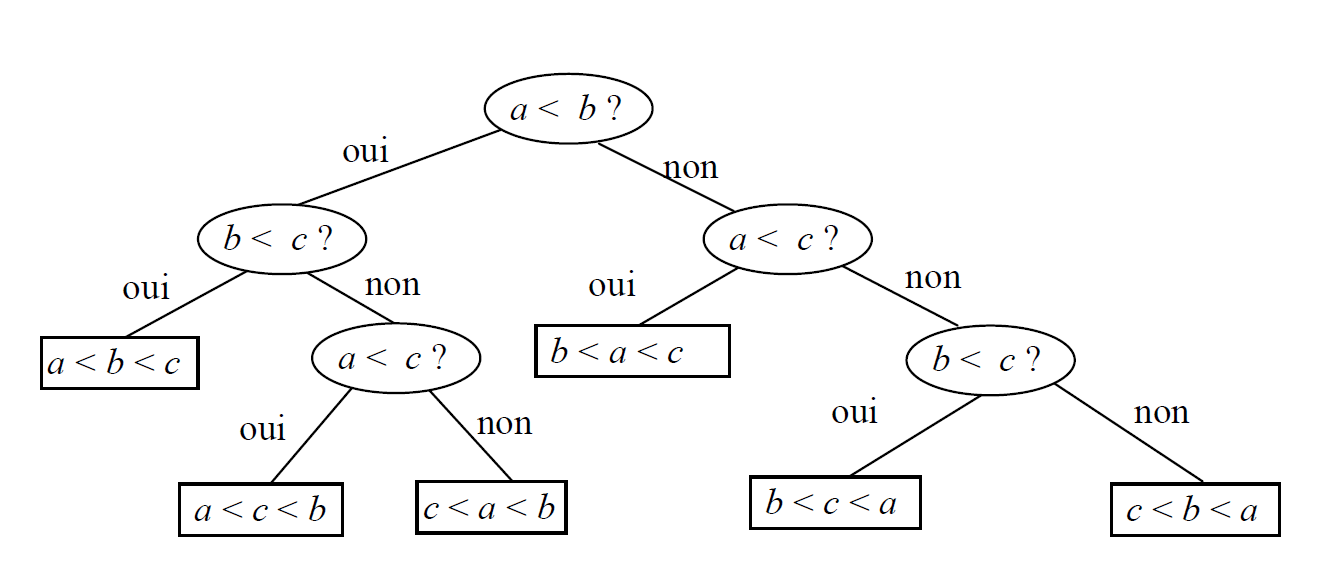
\includegraphics[width=.85\textwidth]{images/C2.png}
\end{center}

\noindent
Cet arbre signifie : la première comparaison faite est « a < b ? ». Si la réponse est oui, la
comparaison suivante est « b < c ? », si la réponse est non c'est « a < c ? ». Lorsqu’une permutation est déterminée, on est dans ce que l'on appelle une feuille de l'arbre. On voit qu'on peut avoir plus
ou moins de chance ; pour deux des permutations, on fait deux comparaisons, pour les quatre
autres, on fait trois comparaisons. Le plus grand nombre de comparaisons est 3, le meilleur est
2 et le nombre moyen de comparaisons est : $(2 \times 2 + 4 \times 3) / 6 \approx 2,67$.





%---------------------------------------------------------------------------
\section{Tri par insertion}
%---------------------------------------------------------------------------
\subsection{Principe}
%---------------------------------------------------------------------------
\noindent
Le tri par insertion est le tri que l'on effectue naturellement, par exemple pour trier un jeu de cartes. On trie les premières puis à chaque nouvelle carte on l'ajoute à l'ensemble déjà trié à la bonne place. Ce tri s'effectue en place, c'est-à-dire qu'il ne demande pas d'autre tableau que celui que l'on trie. 
Son coût en mémoire est donc constant si on ne compte pas la place occupée par les données.

\begin{exemple}
\begin{Objectif}
\noindent
L'objectif de cet exemple est de trier "à la main" la liste L=[7,6,3,5,4,2,1,8] par insertion.
On choisira comme clef (nouvel élément à trier) le premier élément non trié.
\end{Objectif}
\vspace{16cm}
\end{exemple}
%---------------------------------------------------------------------------
\subsection{Implémention}
%---------------------------------------------------------------------------
Un algorigramme du tri par insertion est :
\begin{center}
\includegraphics[width=.65\textwidth]{images/tri_insertion.png}
\end{center}

\begin{exemple}
\noindent
Dans le tri de la liste L=[7,6,3,5,4,2,1,8] utilisant l'algorigramme ci-contre, indiquer chaque changement de la liste L.
\vspace{22cm}
\end{exemple}

\begin{exemple}
\vspace{23cm}
\end{exemple}

\begin{Ques}
\noindent
Ecrire la fonction tri\_insertion qui admet une liste en argument et qui retourne la liste triée. La 
méthode par insertion sera utilisée.
\end{Ques}
\begin{py}
\begin{python}
def tri_insertion(L):

























	return L
\end{python}
\end{py}
%---------------------------------------------------------------------------
\subsection{Complexité}
%---------------------------------------------------------------------------
\noindent
On note $n$ la longueur de la liste L
La fonction tri\_insertion(L) effectue des comparaisons et des affectations (le nombre d'affectation est du même ordre que celui des comparaisons). Lorsque la boucle while insère l'élément $L[i]$ à la position $i-k$, elle
effectue $2(k+1)$ comparaisons. 
\\
\\
\noindent
Dans le meilleur des cas le tableau est déjà trié. 
La valeur clef est donc forcément plus grande que toutes les précédentes. Dès la première comparaison on s'arrête: 
$k$ vaut $0$.
Soit deux comparaisons par boucle while réalisée, il y a donc $2(n-1)$ comparaisons à effectuer au total. La complexité est donc de classe linéaire : $C(n)=O(n)$.
\\
\\
\noindent
Dans le pire des cas, le tableau est trié à l’envers. La valeur clef est donc forcément plus petite que toutes les précédentes.
Il faut donc comparer et décaler toutes les valeurs précédentes jusqu'à mettre la valeur clé en première position:  $k$ vaut $i$, avec $i$ qui varie de $1$ à
$n-1$.
On en déduit donc un nombre total de $2 \times \frac{n \times (n-1)}{2}$ comparaisons.
La complexité est donc de classe quadratique : $C(n)=O(n^2)$.


\begin{center}
\begin{tabular}{|c|c|c|c|}
\hline 
\rule[-1ex]{0pt}{2.5ex}  & meilleur cas & moyenne & pire cas \\ 
\hline 
\rule[-1ex]{0pt}{2.5ex} comparaisons & $n$ & $n^2/4$ & $n^2/2$ \\ 
\hline 
\rule[-1ex]{0pt}{2.5ex} affectations & $n$ & $n^2/4$ & $n^2/2$ \\ 
\hline 
\end{tabular} 
\end{center}
%---------------------------------------------------------------------------
\section{Tri rapide (quicksort)}
%---------------------------------------------------------------------------
\subsection{Principe}
%---------------------------------------------------------------------------
\noindent
L’algorithme fait partie de la catégorie des algorithmes « diviser pour régner ».\\
\noindent
A chaque appel de la fonction tri on choisit une valeur "pivot", par exemple le premier élément. On effectue une partition des éléments à trier. Un premier groupe est constitué de valeurs inférieures au pivot et un deuxième avec les valeurs supérieures.
Le pivot est alors placé définitivement dans le tableau.\\
\noindent
On traite alors chacun des groupes de façon indépendante. On peut les traiter avec le même algorithme (méthode récursive).
\begin{exemple}
\begin{Objectif}
\noindent
L'objectif de cet exemple est de trier "à la main" la liste L=[3,6,8,5,4,2,1,7] par la méthode de tri rapide.
On choisira comme pivot le premier élément de chaque groupe.
\end{Objectif}
\vspace{8cm}
\end{exemple}
%---------------------------------------------------------------------------
\subsection{Implémention}
%---------------------------------------------------------------------------
\noindent
L'implémentation proposé prendra comme pivot le premier élément de chaque liste. On pourrait bien sûr prendre 
un autre pivot, ou le choisir aléatoirement.\\
\noindent
Afin d'implémenter l'algorithme de tri rapide, nous allons décomposer cet algorithme en 
plusieurs fonctions.
%---------------------------------------------------------------------------
\subsubsection{Fonction echange(L,i,j)}
%---------------------------------------------------------------------------
\noindent
Cette fonction permet d'échanger les éléments L[i] et L[j] de la liste L.
\begin{py}
\begin{python}
def echange(L,i,j):
L[i],L[j]=L[j],L[i]
\end{python}
\end{py}
%---------------------------------------------------------------------------
\subsubsection{Fonction partition(L,debut,fin)}
%---------------------------------------------------------------------------
\noindent
Cette fonction place correctement le pivot L[debut] dans la liste L[debut:fin] et retourne sa position. Attention, dans la liste L[debut:fin], L[debut] est inclus et L[fin] est exclus. Cette fonction est décrite par l'algorigramme suivant. La position du pivot est mémorisée dans la variable m.
\begin{center}
\includegraphics[width=.7\textwidth]{images/tri_rapide.png}
\end{center}
\newpage
\begin{exemple}
\noindent
Dans l'appel de la fonction partition utilisant l'algorigramme ci-contre, indiquer les étapes du 
placement du premier pivot dans la liste L=[3,6,8,5,4,2,1,7].
\vspace{22cm}
\end{exemple}


\begin{Ques}
\noindent
Ecrire la fonction partition(L,debut,fin).
\end{Ques}
\begin{py}
\begin{python}
def partition(L,debut,fin):





































	return m
\end{python}
\end{py}
%---------------------------------------------------------------------------
\subsubsection{Fonction tri\_rapide(L)}
%---------------------------------------------------------------------------
\noindent
La fonction tri\_rapide(L) sera implémentée de manière récursive puisque la méthode de tri rapide coupe en deux 
la liste à trier après avoir placer le pivot. Pour cela, nous allons écrire la fonction tri\_rapide\_rec(L,debut,fin) 
qui trie la liste tri\_rapide(L) de manière récursive.
\begin{Ques}
\noindent
Ecrire les fonctions tri\_rapide\_rec(L,debut,fin) et tri\_rapide(L).
\end{Ques}
\begin{py}
\begin{python}
def tri_rapide_rec(L,debut,fin)























def tri_rapide(L):






	return L
\end{python}
\end{py}
%---------------------------------------------------------------------------
\subsection{Complexité}
%---------------------------------------------------------------------------
%---------------------------------------------------------------------------
\subsubsection{Comparaisons}
%---------------------------------------------------------------------------
\noindent
On note $n$ le nombre d'éléments de la liste L.
La fonction partition(L,debut,fin) fait toujours exactement $fin-debut-1$ comparaisons. Si la fonction
partition(L,debut,fin) détermine un segment de longueur $K$ et un autre de longueur $n-1-K$, la fonction
tri\_rapide\_rec(L,debut,fin) va donc effectuer $n-1$ comparaisons par l'intermédiaire de partition,
puis d'autres comparaisons par l'intermédiaire des deux appels récursifs à tri\_rapide\_rec. Le pire des
cas correspond à $K = 0$, ce qui donne, en notant C(n) la complexité du tri d'une liste
de longueur $n$, l'équation de récurrence suivante:
$$C(n) = n-1 + C(n-1)$$,
\noindent
d’où $C(n) \sim \frac{n^2}{2}$. Le meilleur des cas correspond à un segment coupé en deux moitiés
égales, c’est-à-dire $K = n/2$. L’équation de récurrence devient
$$C(n) = n-1 + 2C(n/2).$$
\noindent
On en déduit facilement $C(n) \sim n log n$.
%---------------------------------------------------------------------------
\subsubsection{Affectations}
%---------------------------------------------------------------------------
\noindent
En ce qui concerne le nombre d'affectations, on note que la fonction partition(L,debut,fin) effectue un
appel à échange initial, autant d'appels à échange que d'implémentations de m, et éventuellement
un dernier appel à échange lorsque $m != debut$. Le meilleur des cas est atteint lorsque le
pivot est toujours à sa place. Il y a alors un seul appel à échange, soit deux affectations. Il est
important de noter que ce cas ne correspond pas à la meilleure complexité en termes de
comparaisons (qui est alors quadratique). Dans le pire des cas, le pivot se retrouve toujours
à la position $fin-1$. La fonction partition effectue alors $2(fin-debut)$ affectations, d'où un total de
$n^2$ affectations.
%---------------------------------------------------------------------------
\subsubsection{Bilan}
%---------------------------------------------------------------------------
\begin{center}
\begin{tabular}{|c|c|c|c|}
\hline 
\rule[-1ex]{0pt}{2.5ex}  & meilleur cas & moyenne & pire cas \\ 
\hline 
\rule[-1ex]{0pt}{2.5ex} comparaisons & $n log n$ & $2 n log n$ & $n^2/2$ \\ 
\hline 
\rule[-1ex]{0pt}{2.5ex} affectations & $2n$ & $2 n log n$ & $n^2$ \\ 
\hline 
\end{tabular} 
\end{center}
%---------------------------------------------------------------------------
\section{Tri par fusion}
%---------------------------------------------------------------------------
\subsection{Principe}
%---------------------------------------------------------------------------
\noindent
Cet algorithme fait aussi partie des algorithmes "diviser pour régner".\\
\noindent
Le principe consiste à couper la liste de départ en deux. On trie chacun des groupes indépendamment. Puis on fusionne les deux groupes en utilisant le fait que chacun des groupes est déjà ordonné.\\
\noindent
Il est possible pour réaliser l'ordonnancement de chacun des groupes d'utiliser à nouveau l'algorithme de tri de façon récursive.

\begin{exemple}
\begin{Objectif}
\noindent
L'objectif de cet exemple est de trier "à la main" la liste L=[7,6,3,5,4,2,1,8] par insertion.
On coupera la liste en 2 parties égales (à un élément près). 
\end{Objectif}
\vspace{10cm}
\end{exemple}

\begin{exemple}
\vspace{3cm}
\end{exemple}
%---------------------------------------------------------------------------
\subsection{Implémention}
%---------------------------------------------------------------------------
\noindent
Afin d'implémenter l'algorithme de tri par fusion, nous allons décomposer cet algorithme en 
plusieurs fonctions.
%---------------------------------------------------------------------------
\subsubsection{Fonction fusion(L1,L2,debut,mediane,fin)}
%---------------------------------------------------------------------------
\noindent
Cette fonction permet de fusionner une liste L1 "triée en deux blocs" en la mémorisant dans la liste L2 :
\begin{itemize}
\item L1 est une liste partiellement triée : L1[debut:mediane] et L1[mediane:fin] sont triées
\item L2 est une liste dans laquelle on va fusionner L1[debut:mediane] et L1[mediane:fin] en les triant. 
Les éléments fusionnés seront affectés dans L2[debut:fin].
\end{itemize}
\noindent
Un algorigamme de cette fonction est :\\
\begin{center}
\includegraphics[width=.78\textwidth]{images/fusion.png}
\end{center}
\newpage
\begin{exemple}
\noindent
Donner le résultat de l'appel de la fonction fusion(L1,L2,0,4,8) avec L1=[3,5,6,7,1,2,4,8] et L2=[7,6,3,5,4,2,1,8] en suivant les 
étapes de l'algorigramme ci-contre.
\vspace{22cm}
\end{exemple}

\begin{Ques}
\noindent
Ecrire la fonction fusion(L1,L2,debut,mediane,fin).
\end{Ques}
\begin{py}
\begin{python}
def fusion(L1,L2,debut,mediane,fin):


































# fin du programme
\end{python}
\end{py}
%---------------------------------------------------------------------------
\subsubsection{Fonction tri\_fusion(L)}
%---------------------------------------------------------------------------
\noindent
La fonction tri\_fusion(L) sera implémentée de manière récursive. Pour cela, nous allons écrire la fonction tri\_fusion\_rec(debut,fin) qui trie les liste L1[debut:mediane] et L1[mediane:fin] de manière récursive puis les fusionne. On 
choisit d'implémenter la fonction tri\_fusion\_rec(debut,fin) à l'intérieur de la fonction tri\_fusion(L).
On définit une liste temporaire, notée tmp dans laquelle on va placer les différentes listes "triées par blocs". Initialement, 
on prendra L = tmp.

\begin{Ques}
\noindent
Ecrire la fonctions tri\_fusion(L).
\end{Ques}
\begin{py}
\begin{python}
def tri_fusion(L):
    tmp=L[:]
    def tri_fusion_rec(debut,fin):







































	return L
\end{python}
\end{py}
%---------------------------------------------------------------------------
\subsection{Complexité}
%---------------------------------------------------------------------------
\noindent
Si on note $C(n)$ (respectivement $f(n)$) le nombre total de comparaisons effectuées par tri\_fusion
(respectivement fusion) pour trier une liste de longueur $n$, on a l'équation de récurrence :
$$C(n) = 2C(n/2) + f(n)$$
car les deux appels récursifs se font sur deux segments de même longueur $n/2$. Dans le
meilleur des cas, la fonction fusion n'examine que les éléments de l'un des deux segments
car ils sont tous plus petits que ceux de l'autre segment. Dans ce cas $f(n) = n/2$ et donc
$C(n) \sim \frac{1}{2} n log n$. Dans le pire des cas, tous les éléments sont examinés par fusion et
donc $f(n) = n-1$, d’où $C(n) \sim n log n$.\\

\noindent
Le nombre d’affectations est le même dans tous les cas : $n$ affectations dans la fonction
fusion (chaque élément est copié de $L1$ vers $L2$) et $n$ affectations effectuées par la copie de a
vers $tmp$. Si on note $A(n)$ le nombre total d’affectations pour trier une liste de longueur
$n$, on a donc
$$A(n) = 2A(n/2) + 2n,$$
d’où un total de $2n log n$ affectations.
\end{document}
